\documentclass[10pt]{article}

\def\Type{LessonCaelan}
\def\TypeNum{Lesson 21}
\def\TypeTitle{Continuous Random Variables}
\def\Semester{Fall 2021} %Not Used 
\def\Course{MATH 1190 \& 1210}

\usepackage{preambleDJ}



%%%%%%%%%%%% BEGIN DOCUMENT %%%%%%%%%%%%%%%
%%%%%%%%%%%% BEGIN DOCUMENT %%%%%%%%%%%%%%%
%%%%%%%%%%%% BEGIN DOCUMENT %%%%%%%%%%%%%%%
%%%%%%%%%%%% BEGIN DOCUMENT %%%%%%%%%%%%%%%
%%%%%%%%%%%% BEGIN DOCUMENT %%%%%%%%%%%%%%%

\begin{document}


\thispagestyle{firstpage}
\pagestyle{otherpages}
\vs{0.5}

%\Heading{MATH 1190 \& 1210 Survey of Calculus I}{\begin{minipage}{0.25\textwidth}\begin{center} Lesson 20\\ Introduction to Probability \end{center}\end{minipage}}

\textbf{Intended Learning Outcomes}
After this lesson, you will be able to 

\begin{itemize}
\item Determine if a random variable is discrete or continuous. (\target{P1}, \target{P2})
\item Define support for a continuous random variable. (\target{P2})
\item List and apply properties of the probability density function of a continuous random variable. (\target{P2})
\item Find the formula and the graph of the cumulative distribution function of a continuous random variable. (\target{P2)}
\end{itemize}

\vspace{-0.5cm}

\hrulefill

\minil
We have seen {\em discrete random variables} have outcomes that are {\em countable}  (e.g. $1$,$2$,$3$, $\dots$.) Frequently there will only be a {\em finite} number of these values.\\
\blue{\bf Example} Last time we saw an example where $X$ was the (random) sum after rolling $2$ six-sided dice. We saw
\itemI{
\item Possible outcomes are $\ds \{ 2,3,4,5,6,7,8,9,10,11,12\}$ (tick marks on $x$-axis below)
\item The {\em probability mass function, $p(x)$} describes the probability for each outcome.  %%Need to add better description. Maybe a step function???
\item The probability of each outcome can also be represented by the areas of each bar in the histogram below, assuming the width of each bar is $1$.
} 
What happens if examine the sum of  many, many, many dice?
~\\
\hs{-.3}\mpageTth{.35}{.35}{.35}[\hs{.15}][\hs{.15}]{
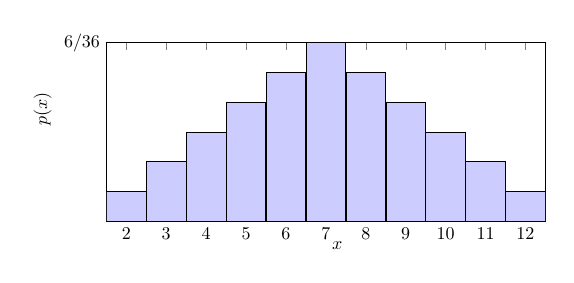
\begin{tikzpicture}[scale=0.65]
\begin{axis}[
%ymin=0, % Ensures bars start from zero
	xtick={1,	2,	3,	4,	5,	6,	7,	8,	9,	10,	11}, % Places x-axis ticks at data points
	xticklabels={
         2,	3,	4,	5,	6,	7,	8,	9,	10,	11,	12
         }, % Custom x-axis labels
	ytick       = {6/36},
	yticklabels =  {$6/36$},
enlarge x limits={.05}, % Adjusts spacing between bars and axis limits
	y label style={anchor=south west},
	ylabel={$p(x)$},
	xlabel = {$x$},
	x label style={anchor=west},
	%xticklabel style = {font=\small}, 
	ymin = 0, ymax = .167,
	width = 4in, height=2in,
	axis line style={->},
]
% \addplot[fill=blue!20] coordinates {(1,0)  (2,0)  (3,0) (4,0) (5,0) (6,0) (7,0) (8,0) (9,0) (10,0) (11,0)};
\addplot[ybar, bar shift=0,   bar width=22pt,  fill=blue!20] plot coordinates {
(1 , 0.02777778)	(2 , 0.05555556)	(3 , 0.08333333)	(4 , 0.11111111)	(5 , 0.13888889)	(6 , 0.16666667)	(7 , 0.13888889)	(8 , 0.11111111)	(9 , 0.08333333)	(10 , 0.05555556)	(11 , 0.02777778)
};
%\addplot[ybar, bar shift=0,   bar width=22pt,  fill=blue] plot coordinates {
%(1 , 0.02777778)	(2 , 0.05555556)	(3 , 0.08333333)	};
%	  \addplot[domain=0.5:1.5,  red, ultra thick, -, ] { 0.02777778 };
\end{axis}
\end{tikzpicture}
\centering
\parbox{1.2\textwidth}{\centering Histogram for Sum of $n=2$ dice}
}{
%
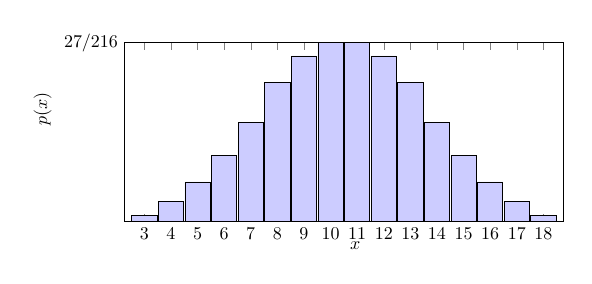
\begin{tikzpicture}[scale=0.65]
\begin{axis}[
%ymin=0, % Ensures bars start from zero
	xtick={1,	2,	3,	4,	5,	6,	7,	8,	9,	10,	11,	12,	13,	14,	15, 16}, % Places x-axis ticks at data points
	xticklabels={
         3,	4,	5,	6,	7,	8,	9,	10,	11,	12,	13,	14,	15,	16,	17, 18
         }, % Custom x-axis labels
	ytick       = {27/216},
	yticklabels =  {$27/216$},
	enlarge x limits={0.05}, % Adjusts spacing between bars and axis limits
	y label style={anchor=south west},
	ylabel={$p(x)$},
	xlabel = {$x$},
	x label style={anchor=west},
	%xticklabel style = {font=\small}, 
	ymin = 0, ymax = .125,
	width = 4in, height=2in,
	axis line style={->},
]
	% \addplot[fill=blue!20] coordinates {(1,0)  (2,0)  (3,0) (4,0) (5,0) (6,0) (7,0) (8,0) (9,0) (10,0) (11,0)};
	\addplot[ybar, bar shift=0,   bar width=14pt,  fill=blue!20] plot coordinates {
	(1 , 0.00462963)	(2 , 0.01388889)	(3 , 0.02777778)	(4 , 0.0462963)	(5 , 0.06944444)	(6 , 0.09722222)	(7 , 0.11574074)	(8 , 0.125)	(9 , 0.125)	(10 , 0.11574074)	(11 , 0.09722222)	(12 , 0.06944444)	(13 , 0.0462963)	(14 , 0.02777778)	(15 , 0.01388889) (16 , 0.00462963)
		};
\end{axis}
\end{tikzpicture}
\parbox{1.3\textwidth}{\centering Histogram for Sum of $n=3$ dice}
}{
%
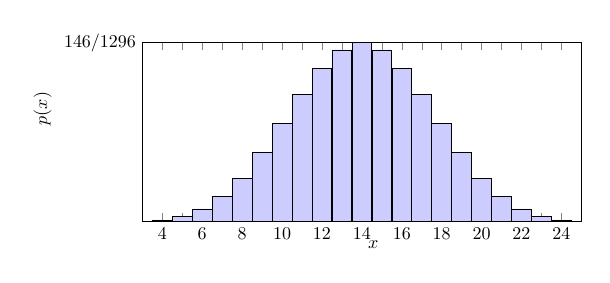
\begin{tikzpicture}[scale=0.65]
\begin{axis}[
	xtick={1,	2,	3,	4,	5,	6,	7,	8,	9,	10,	11,	12,	13,	14,	15,	16,	17,	18,	19,	20,	21}, % Places x-axis ticks at data points
	xticklabels={
         4,	,	6,	,	8,	,	10,	,	12,	,	14,	,	16,	,	18,	,	20,	,	22,	,	24
         }, % Custom x-axis labels
	ytick       = {146/1296},
	yticklabels =  {$146/1296$},
	y label style={anchor=south west},
ylabel={$p(x)$},
	xlabel = {$x$},
	enlarge x limits={0.05}, % Adjusts spacing between bars and axis limits
	x label style={anchor=west},
	%xticklabel style = {font=\small}, 
	ymin = 0, ymax = .113,
	width = 4in, height=2in,
	axis line style={->},
]
	% \addplot[fill=blue!20] coordinates {(1,0)  (2,0)  (3,0) (4,0) (5,0) (6,0) (7,0) (8,0) (9,0) (10,0) (11,0)};
	\addplot[ybar, bar shift=0, bar width=11pt,  fill=blue!20] plot coordinates {
	(1 , 0.0007716)	(2 , 0.00308642)	(3 , 0.00771605)	(4 , 0.0154321)	(5 , 0.02700617)	(6 , 0.04320988)	(7 , 0.0617284)	(8 , 0.08024691)	(9 , 0.09645062)	(10 , 0.10802469)	(11 , 0.11265432)	(12 , 0.10802469)	(13 , 0.09645062)	(14 , 0.08024691)	(15 , 0.0617284)	(16 , 0.04320988)	(17 , 0.02700617)	(18 , 0.0154321)	(19 , 0.00771605)	(20 , 0.00308642)	(21 , 0.0007716)
	};
\end{axis}
\end{tikzpicture}
\parbox{1.4\textwidth}{\centering Histogram for Sum of $n=4$ dice}    
}

\hs{-.3}\mpageTth{.35}{.4}{.35}[\hs{.15}][\hs{.15}]{
\parbox{1.5\textwidth}{\centering \hs{3.5}\,}   
}{
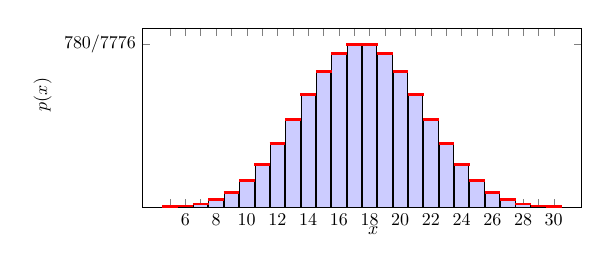
\begin{tikzpicture}[scale=0.65]
\begin{axis}[
%ymin=0, % Ensures bars start from zero
	xtick={1,	2,	3,	4,	5,	6,	7,	8,	9,	10,	11,	12,	13,	14,	15,	16,	17,	18,	19,	20,	21,	22,	23,	24,	25,	26}, % Places x-axis ticks at data points
	xticklabels={
         ,	6,	,	8,	,	10,	,	12,	,	14,	,	16,	,	18,	,	20,	,	22,	,	24,	,	26,	,	28,	,	30,
         }, % Custom x-axis labels
	ytick       = {780/7776},
	yticklabels =  {$780/7776$},
	enlarge x limits={.05}, % Adjusts spacing between bars and axis limits
	y label style={anchor=south west},
	ylabel={$p(x)$},
	xlabel = {$x$},
	x label style={anchor=west},
	%xticklabel style = {font=\small}, 
	ymin = 0, ymax = .1103,
	width = 4in, height=2in,
	axis line style={->},
]
	% \addplot[fill=blue!20] coordinates {(1,0)  (2,0)  (3,0) (4,0) (5,0) (6,0) (7,0) (8,0) (9,0) (10,0) (11,0)};
	\addplot[ybar, bar shift=0,   bar width=8pt,  fill=blue!20] plot coordinates {
(	(1 , 0.0001286)	(2 , 0.000643)	(3 , 0.00192901)	(4 , 0.00450103)	(5 , 0.00900206)	(6 , 0.0162037)	(7 , 0.02636317)	(8 , 0.03922325)	(9 , 0.05401235)	(10 , 0.06944444)	(11 , 0.08371914)	(12 , 0.0945216)	(13 , 0.10030864)	(14 , 0.10030864)	(15 , 0.0945216)	(16 , 0.08371914)	(17 , 0.06944444)	(18 , 0.05401235)	(19 , 0.03922325)	(20 , 0.02636317)	(21 , 0.0162037)	(22 , 0.00900206)	(23 , 0.00450103)	(24 , 0.00192901)	(25 , 0.000643)	(26 , 0.0001286)
	};
	 % \addplot[ domain=0:26,  red, ultra thick, <->, ] {1/sqrt(2*pi*(3.85)^2)*e^(-(x-13.5)^2/(2*(3.85)^2))  };
	 \addplot[domain=0.5:1.5, red, ultra thick] {0.0001286};
\addplot[domain=1.5:2.5, red, ultra thick] {0.000643};
\addplot[domain=2.5:3.5, red, ultra thick] {0.00192901};
\addplot[domain=3.5:4.5, red, ultra thick] {0.00450103};
\addplot[domain=4.5:5.5, red, ultra thick] {0.00900206};
\addplot[domain=5.5:6.5, red, ultra thick] {0.0162037};
\addplot[domain=6.5:7.5, red, ultra thick] {0.02636317};
\addplot[domain=7.5:8.5, red, ultra thick] {0.03922325};
\addplot[domain=8.5:9.5, red, ultra thick] {0.05401235};
\addplot[domain=9.5:10.5, red, ultra thick] {0.06944444};
\addplot[domain=10.5:11.5, red, ultra thick] {0.08371914};
\addplot[domain=11.5:12.5, red, ultra thick] {0.0945216};
\addplot[domain=12.5:13.5, red, ultra thick] {0.10030864};
\addplot[domain=13.5:14.5, red, ultra thick] {0.10030864};
\addplot[domain=14.5:15.5, red, ultra thick] {0.0945216};
\addplot[domain=15.5:16.5, red, ultra thick] {0.08371914};
\addplot[domain=16.5:17.5, red, ultra thick] {0.06944444};
\addplot[domain=17.5:18.5, red, ultra thick] {0.05401235};
\addplot[domain=18.5:19.5, red, ultra thick] {0.03922325};
\addplot[domain=19.5:20.5, red, ultra thick] {0.02636317};
\addplot[domain=20.5:21.5, red, ultra thick] {0.0162037};
\addplot[domain=21.5:22.5, red, ultra thick] {0.00900206};
\addplot[domain=22.5:23.5, red, ultra thick] {0.00450103};
\addplot[domain=23.5:24.5, red, ultra thick] {0.00192901};
\addplot[domain=24.5:25.5, red, ultra thick] {0.000643};
\addplot[domain=25.5:26.5, red, ultra thick] {0.0001286};
\end{axis}
\end{tikzpicture}
\parbox{1.2\textwidth}{\centering Histogram for Sum of $n=5$ dice}    
}{
\begin{tikzpicture}[scale=0.65]
\begin{axis}[
%ymin=0, % Ensures bars start from zero
	xtick=\empty, %{1,	2,	3,	4,	5,	6,	7,	8,	9,	10,	11,	12,	13,	14,	15,	16,	17,	18,	19,	20,	21,	22,	23,	24,	25,	26}, % Places x-axis ticks at data points
	xticklabels={10,18}, % Custom x-axis labels
	ytick       = \empty, %{780/7776},
	yticklabels =  {$780/7776$},
enlarge x limits={.05}, % Adjusts spacing between bars and axis limits
	y label style={anchor=south west},
	ylabel={$p(x)$},
	xlabel = {$x$},
	x label style={anchor=west},
	xticklabel style = {font=\small}, 
	ymin = 0, ymax = .1103,
	width = 4in, height=2in,
	axis line style={->},
]
	  \addplot[ name path=f, domain=0:26,  red, ultra thick, <->, ] {1/sqrt(2*pi*(3.85)^2)*e^(-(x-13.5)^2/(2*(3.85)^2))  };
	   \path[name path=axis] (0,0) -- (26,0);
	    \addplot [
                    thick,
                    color=blue!20,
                    fill=blue!20, 
                    ]
                    fill between[
                    of=f and axis,
                    soft clip={domain=0:26},
                    ];
\end{axis}
\end{tikzpicture}
\parbox{1\textwidth}{\centering Histogram for Sum of $n\to\infty$ dice}   
}
\vs{.5}
A {\em continuous probability distribution} is continuous because the set of outcomes of an experiment
is continuous. (e.g. measuring the height of a person, determining the wait time at the DMV,
weighing a Roots Bowl, etc).
\itemI{
\item Possible outcomes are an interval: $\ds (-\infty,\infty)$, $([0,1]$, $[0,100]$, etc.
\item The {\em probability density function} $p(x)$ is continuous and is used to find the probability for a range of outcomes.
\item The probability of between two values is equivalent to the area between $p(x)$ and the horizontal axis.
}


\newpage

\textbf{\color{blue} Warm Up}\exercise{\bf\color{Orange}P1, P2} Determine whether each of the random variable in the following scenarios is discrete or continuous.

\begin{enumerate}[label=(\alph*)]
\item $X$ is the (random)  number of arrivals at an emergency room from midnight to 6am on a given day.

\vfill
\item $T$ is the (random)  temperature of a cup of coffee from a coffee shop.


\vfill 

\item $B$ is the number of boys in a randomly-selected family with 3 children.

\vfill
\end{enumerate}

%%%%%%%%%
\newpage%
%%%%%%%%%
\blue{\bf Key Properties of  Continuous Random Variables}\\
\mpageT{.5}{.5}[\hs{.1}]{
\centering
\blue{ \bf Discrete Random Variables}
}{
\centering
\blue{ \bf Continuous Random Variables}\\
}%\vs{-.2}
\itemNIN{
\mpageT{.5}{.5}[\hs{.2}]{
\item {\bf Discrete Example: } The random variable $X$ is the sum from randomly rolling two $4$-sided dice
}{
\item \blue{\bf Continuous}\example The random variable $T$ is the (random) wait time until the bus arrives  at the 
amphitheater on McIntyre. Buses arrive every $30$ minutes with evenly distributed probability (a uniform distribution)
}
\vs{.0}\\
\mpageT{.5}{.5}[\hs{.2}]{
\item The {\em Sample Space of $X$}: $S_X=\{2,3,4,5,6,7,8\}$
}{
\item The {\em Support of $T$}: $S_T=$ 
\\\\
$S=[a,b]$:  $[a,b]$ is smallest interval where $p(t)> 0$
}
\vs{.2}\\
\mpageT{.5}{.5}[\hs{.2}]{
\item {\bf Probability Mass Function}:  $p(x)$.\\
{ \em Two Properties:}
\enum{
\item $0\leq p(x)\leq 1$ where $x\in S_X$\vs{.3}
\item $\ds \sum_{k\in S_X}P[X=k] = \sum_{k=2}^8 P[X=k]=\sum_{k=2}^8 p(k)=1$
}
%
}{
\item {\bf Probability Density Function (PDF)}: $p(t)$.\\
{ \em Two Properties:}
\enum{
\item \mbox{}\vs{.3}~\\
\item \mbox{} 
}
\vs{.1}
}

\mpageT{.5}{.5}[\hs{.2}]{
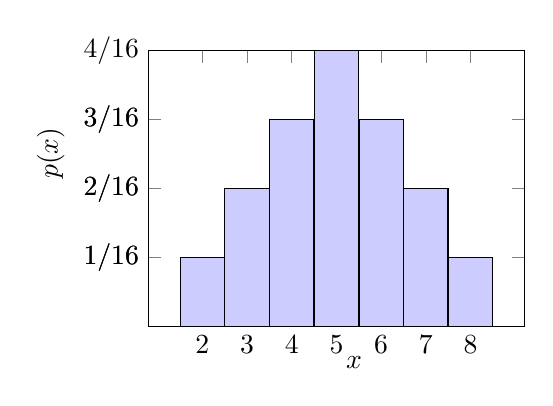
\begin{tikzpicture}
\begin{axis}[
%ymin=0, % Ensures bars start from zero
	xtick={1,	2,	3,	4,	5,	6,	7}, % Places x-axis ticks at data points
	xticklabels={
         2,	3,	4,	5,	6,	7,	8
         }, % Custom x-axis labels
ytick       = {1/16, 2/16, 3/16,4/16,3/16,2/16,1/16},
yticklabels =  {$1/16$, $2/16$, $3/16$,$4/16$,$3/16$,$2/16$,$1/16$},
enlarge x limits={.2}, % Adjusts spacing between bars and axis limits
	y label style={anchor=south west},
	ylabel={$p(x)$},
	xlabel = {$x$},
	x label style={anchor=west},
	%xticklabel style = {font=\small}, 
	ymin = 0, ymax = .25,
	width = 2.5in, height=2in,
	   axis line style={->},
]
% \addplot[fill=blue!20] coordinates {(1,0)  (2,0)  (3,0) (4,0) (5,0) (6,0) (7,0) (8,0) (9,0) (10,0) (11,0)};
\addplot[ybar, bar shift=0,   bar width=16pt,  fill=blue!20] plot coordinates {
(1,.0625)  (2,.125) (3,.1875) (4,.25) (5,.1875) (6,.125) (7,.0625) 
};
\end{axis}
\end{tikzpicture}
}{
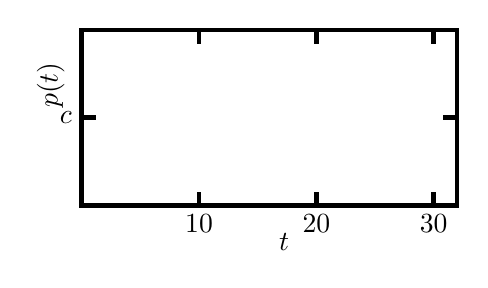
\begin{tikzpicture}
\begin{axis}[
	x label style={anchor=west},
xlabel={$t$},
xtick       = {10,20,30},
%xticklabels = {$10$,$20$,$30$},
xticklabel style={anchor=north},
y label style={anchor=west},
ylabel={$p(t)$},
%ytick=\empty,
%ytick       = {1/30},
ytick={0.05},
yticklabels = {$c$},
samples     = 320,
%domain      = -2.5:2.5,
%restrict y to domain=-6.5:6.5,
xmin =0, xmax = 32,
ymin = 0, ymax = .1,
axis line style = { ultra thick, -},
every major tick/.append style={ultra thick, black, major tick length=5pt},
width=2.5in, height=1.5in
%  grid=both, grid style=solid
]
  %\addplot[domain=0:30, blue, ultra thick, mark=none]{.05};
%    \addplot[domain=0:5, blue, ultra thick, mark=none]{1/25*x};
%     \addplot[domain=5:10, blue, ultra thick, mark=none]{-1/25*x+2/5};
\end{axis}
\end{tikzpicture}
}
}
\tasksA{2}{
\task What is the support of $T$?





\task What is the value of $c$ in the above graph?. Hint: Consider how property $\#2$ for continuous random variables might be helpful.\vs{1}


\task Use $p(t)$ and an integral to find $P(T\leq 10)$, the probability that this person waits for no more than 10 minutes.\\

}
\newpage


\exercise{\bf\color{Orange}P2  }
Let $X$ be a continuous random variable with probability density function given by:
\[
p(x) = 
\begin{cases} 
cx & \text{for } 0 \leq x \leq 2, \\
0 & \text{otherwise}.
\end{cases}
\]
\tasksA{2}{

\task Find the support of $X$.\\ $S=\unlineb{2}{}$


\task Find the value of the constant $c$ making $p(x)$ a valid probability density function. Then sketch $p(x)$.

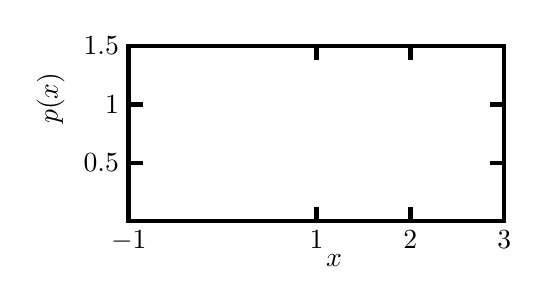
\begin{tikzpicture}
\begin{axis}[
	x label style={anchor=west},
xlabel={$x$},
xtick       = {-1,1,2,3},
xticklabels = {$-1$,$1$,$2$,$3$},
xticklabel style={anchor=north},
y label style={anchor=south west},
ylabel={$p(x)$},
ytick       = {.5,1,1.5},
yticklabels = {$0.5$,$1$,$1.5$},
samples     = 320,
xmin =-1, xmax = 3,
ymin = 0, ymax = 1.5,
axis line style = { ultra thick, -},
every major tick/.append style={ultra thick, black, major tick length=5pt},
width=2.5in, height=1.5in
%  grid=both, grid style=solid
]
%\addplot[domain=0:2, red, ultra thick, mark=none]{1/2*x};
%\addplot[domain=-1:0, red, ultra thick, mark=none]{0};
%\addplot[domain=2:3, red, ultra thick, mark=none]{0};
%\filldraw[fill=white, thick] (2,0) circle (2pt);
\end{axis}
\end{tikzpicture}

\vs{2.5}
\task Using the value of $c$ you found in b), find\\ $P(X\leq 3/2)$, i.e. the probability that $X$ takes on a value less than or equal to $1.5$.

\task Give an example of an interval $[0,b]$ that $X$ has a $25\%$ chance of falling in. Show your answer is correct.
}

%%%%%%%%%
\newpage%
%%%%%%%%%

{\bf\color{blue}Mini-lecture.} The {\bf cumulative distribution function} (CDF) of a continuous random variable $X$ measures how much probability has accumulated up to a given point.    Informally, it is the ``probability-so-far" function
$$F(x) = \unlineb{2}{}$$
\vs{.3}

\example{\bf\color{Orange}P2} Let's continue with the previous \blue{\bf Exercise B} with utilizing the probability density function and graph below.\\
\mpageT{.5}{.5}{\centering
$$
p(x) = 
\begin{cases} 
cx & \text{for } 0 \leq x \leq 2, \\
0 & \text{otherwise}.
\end{cases}
$$
}{\centering
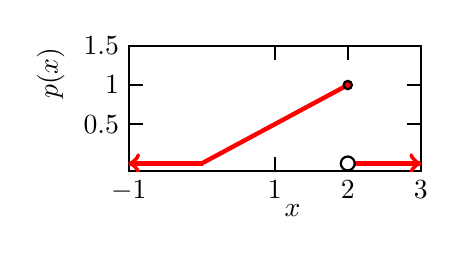
\begin{tikzpicture}
\begin{axis}[
	x label style={anchor=west},
xlabel={$x$},
xtick       = {-1,1, 2,3},
xticklabels = {$-1$,$1$,$2$,$3$},
xticklabel style={anchor=north},
y label style={anchor=south west},
ylabel={$p(x)$},
ytick       = {.5,1,1.5},
yticklabels = {$0.5$,$1$,$1.5$},
samples     = 320,
xmin =-1, xmax = 3,
ymin = -.1, ymax = 1.5,
axis line style = {  thick, ->},
every major tick/.append style={ thick, black, major tick length=5pt},
width=2.083in, height=1.25in
]
	\addplot[domain=0:2, red, ultra thick, mark=none]{x/2};
\addplot[domain=2:3, red, ultra thick, ->]{0};
	\addplot[domain=-1:0, red, ultra thick, <-]{0};
	          \filldraw[fill=white, thick] (2,0) circle (2.5pt);
	                    \filldraw[fill=red, thick] (2,1) circle (1.5pt);
\end{axis}
\end{tikzpicture}
}
\tasksA{2}{
\task Based on the definition we just learned, what is the cumulative distribution function $F(x)$ of the random variable $X$? You will want to use the value of $c$ found in the previous exercise.

\task Find $F(3/2)$ and $F(2)$. These should be consistent with work done on the previous exercise.\vs{2}

\task* Sketch the graph of $F(x)$. 

\mpageT{.5}{.5}{\centering
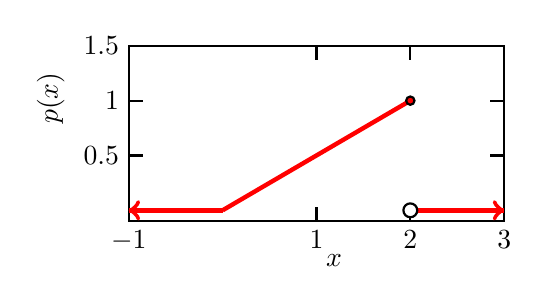
\begin{tikzpicture}
\begin{axis}[
	x label style={anchor=west},
xlabel={$x$},
xtick       = {-1,1, 2,3},
xticklabels = {$-1$,$1$,$2$,$3$},
xticklabel style={anchor=north},
y label style={anchor=south west},
ylabel={$p(x)$},
ytick       = {.5,1,1.5},
yticklabels = {$0.5$,$1$,$1.5$},
samples     = 320,
xmin =-1, xmax = 3,
ymin = -.1, ymax = 1.5,
axis line style = {  thick, ->},
every major tick/.append style={ thick, black, major tick length=5pt},
width=2.5in, height=1.5in
]
	\addplot[domain=0:2, red, ultra thick, mark=none]{x/2};
\addplot[domain=2:3, red, ultra thick, ->]{0};
	\addplot[domain=-1:0, red, ultra thick, <-]{0};
	          \filldraw[fill=white, thick] (2,0) circle (2.5pt);
	                    \filldraw[fill=red, thick] (2,1) circle (1.5pt);
\end{axis}
\end{tikzpicture}
}{\centering
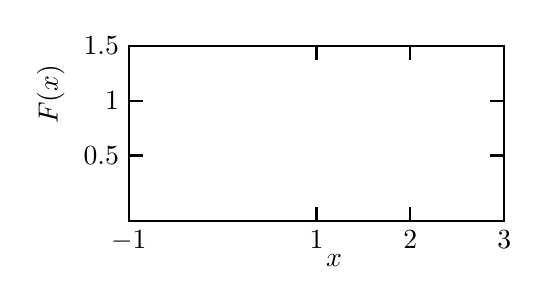
\begin{tikzpicture}
\begin{axis}[
	x label style={anchor=west},
xlabel={$x$},
xtick       = {-1, 1, 2,3},
xticklabels = {$-1$, $1$,$2$,$3$},
xticklabel style={anchor=north},
y label style={anchor=south west},
ylabel={$F(x)$},
ytick       = {.5,1,1.5},
yticklabels = { $0.5$,$1$ ,$1.5$},
samples     = 320,
xmin =-1, xmax = 3,
ymin = -.1, ymax = 1.5,
axis line style = {  thick, ->},
every major tick/.append style={ thick, black, major tick length=5pt},
width=2.5in, height=1.5in
]
\end{axis}
\end{tikzpicture}
}
\task* Find $P(1/2\leq X\leq 3/2)$ two ways:
}
\tasksI{2}{
\task Consider how the graph of $p(x)$ relates to this probability. 

\task Consider how $F(x)$ can be used to find this probability.
}

\newpage
\exercise{\bf\color{Orange}P2}
The probability density function of a random variable $X$ is given below:
\[
p(x) = 
\begin{cases} 
3x^2 & \text{for } 0 \leq x \leq 1, \\
0 & \text{otherwise},
\end{cases}
\]
\tasksA{2}{
\task* Find and graph the cumulative distribution function $F(x)$.\vs{2}\\
\mpageT{.6}{.4}{
\,
}{
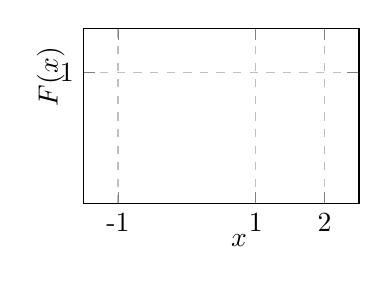
\begin{tikzpicture}
\begin{axis}[
xlabel = {$x$},
x label style={anchor=west},
ylabel = {$F(x)$},
y label style={anchor=west},
xtick       = {-1,1,2},
xticklabels = {-1,1,2},
ytick       = {1,2},
yticklabels = {1,2},
samples     = 160,
domain      = -1:3,
restrict y to domain=-0.1:4,
xmin = -1.5, xmax = 2.5,
ymin = -0.5, ymax = 1.5,
width = 2in, height=1.5in,
grid=both, grid style=dashed
]
\end{axis}
\end{tikzpicture}
}
\task Utilize $F(x)$ to find $P(X\leq 1/4)$

\task What is $P(X>1/4)$? Consider how property $\#2$ of a continuous random variable might be helpful.\vs{1.5}

\task What is $P(1/4\leq X \leq 1/2)$?

\task Find $b$ so that $P(X\leq b)=\dfrac{8}{27}$

}


%%%%%%%%%
\newpage%
%%%%%%%%%

\exercise{\bf\color{Orange}P2}
%%%%%EXERCISE D%%%%%%%%%%%%%%%%
The probability density function of a random variable $Z$ and its graph are given below:
\mpageT{.5}{.5}{
\[
p(z) = 
\begin{cases} 
\dfrac{3}{14}  \sqrt{z}& \text{for } 1 \leq z \leq 4, \\
0 & \text{otherwise}
\end{cases}
\]
}{\centering
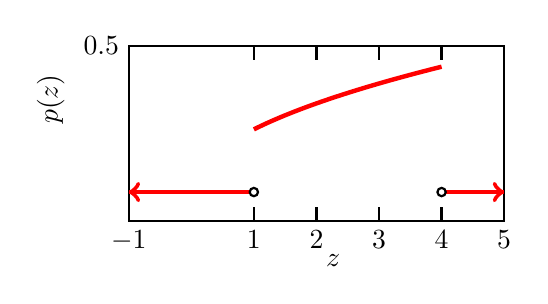
\begin{tikzpicture}
\begin{axis}[
	x label style={anchor=west},
xlabel={$z$},
xtick       = {-1,1,2,3,4,5},
xticklabels = {$-1$,$1$,$2$,$3$,$4$,$5$},
xticklabel style={anchor=north},
y label style={anchor=south west},
ylabel={$p(z)$},
ytick       = {.5, 9/16,1,1.5},
yticklabels = {$0.5$,,$1$,$1.5$},
samples     = 320,
xmin =-1, xmax = 5,
ymin = -.1, ymax = .5,
axis line style = {  thick, ->},
every major tick/.append style={ thick, black, major tick length=5pt},
width=2.5in, height=1.5in
]
\addplot[domain=1:4, red, ultra thick, mark=none]{ 3/14*sqrt(x) };
\addplot[domain=4:5, red, ultra thick, ->]{0};
    \addplot[domain=-1:1, red, ultra thick, <-]{0};
     \filldraw[fill=white, thick] (1,0) circle (1.5pt);
                      \filldraw[fill=white, thick] (4,0) circle (1.5pt);
\end{axis}
\end{tikzpicture}
}

\tasksA{2}{
\task Find the cumulative distribution function $F(z)$
\task Find $P( Z \leq 9/4)$

}
\vs{3}

{\bf\color{blue}Extra Practice 1.} \ltrm{\bf\color{Orange}P2}
The PDF of the continuous random variable $X$ is given below:\\

\

\,\hfill
%
\begin{minipage}[t][0.5in]{0.25\textwidth}
$
p(x) = 
\begin{cases} 
1 & \text{for } 0 \leq x \leq 1, \\
0 & \text{otherwise},
\end{cases}
$
\end{minipage}
%
\hfill
%
\begin{minipage}[t][0.5in]{0.25\textwidth}
\,\\[-0.5in]
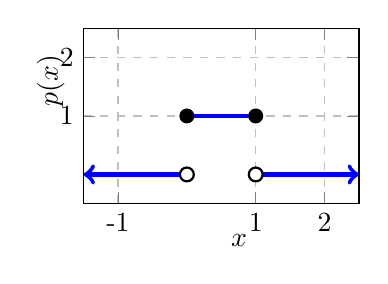
\begin{tikzpicture}
\begin{axis}[
%    axis y line = left,
%    axis x line = bottom,
xlabel = {$x$},
x label style={anchor=west},
ylabel = {$p(x)$},
y label style={anchor=west},
xtick       = {-1,1,2},
xticklabels = {-1,1,2},
ytick       = {1,2},
yticklabels = {1,2},
samples     = 160,
domain      = -1:3,
xmin = -1.5, xmax = 2.5,
ymin = -0.5, ymax = 2.5,
width = 2in, height=1.5in,
grid=both, grid style=dashed
]
\draw[ultra thick,blue,<-] (-1.5,0) -- (0,0);
\draw[ultra thick,blue] (0,1) -- (1,1);
\draw[ultra thick,blue,->] (1,0) -- (2.5,0);
\filldraw (0,1) circle (2.5pt);
\filldraw (1,1) circle (2.5pt);
\filldraw[fill=white, thick] (1,0) circle (2.5pt);
\filldraw[fill=white, thick] (0,0) circle (2.5pt);
\end{axis}
\end{tikzpicture}
\end{minipage}
%
\hfill\,\\

\begin{itemize}
\item[(a)] Find the CDF $F(x)$ of $X$.\vs{1.25}



\end{itemize}

\begin{minipage}[t]{0.5\textwidth}
\begin{itemize}
\item[(b)] Sketch the graph of the CDF $F(x)$.

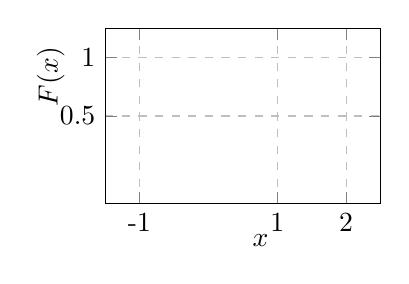
\begin{tikzpicture}
\begin{axis}[
xlabel = {$x$},
x label style={anchor=west},
ylabel = {$F(x)$},
y label style={anchor=west},
xtick       = {-1,1,2},
xticklabels = {-1,1,2},
ytick       = {1,2},
yticklabels = {0.5,1},
samples     = 160,
domain      = -1:3,
xmin = -1.5, xmax = 2.5,
ymin = -0.5, ymax = 2.5,
width = 2in, height=1.5in,
grid=both, grid style=dashed
]
\end{axis}
\end{tikzpicture}
\end{itemize}
\end{minipage}
%
\begin{minipage}[t]{0.45\textwidth}
\begin{itemize}
\item[(c)] Find the number $m$ for which $P(X<m)=0.5$. ({\bf Note:} this number $m$ is called the {\bf median} of $X$.)

\end{itemize}
\end{minipage}

\newpage

{\bf\color{blue}Extra Practice 2.} \ltrm{\bf\color{Orange}P2}Consider the following probability density function for a random variable $X$:
\[
p(x) = 
\begin{cases} 
cx(1 - x) & \text{for } 0 \leq x \leq 1, \\
0 & \text{otherwise}.
\end{cases}
\]
\tasksA{2}{
\task Find the value of $c$ making $f$ a valid probability density function.


\task Suppose you know $X$ has a 75\% chance to fall in the interval $[a,1]$. Find $a$.\vs{4}



%%%%%%%%%
%\newpage%
%%%%%%%%%

\task* Suppose you know $X$ has a 25\% chance to fall in the interval $[0,b]$. Find $b$.



}

\newpage
{\bf\color{blue}Extra Practice 3.} \ltrm{\bf\color{Orange}P2}
Suppose we want to analyze the fishing industry in a small town. Each day, the boats bring back at least 2 tons of fish, but never more than 8 tons.

Suppose $X$ is the continuous random variable for the amount of fish brought back by the boats on a day. The following figure shows the the probability density function $p(x)$ of $X$. 

\begin{center}
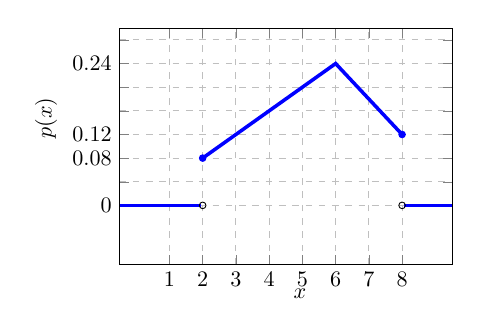
\begin{tikzpicture}[scale=.8]
\begin{axis}[
x label style={anchor=west},
xlabel={$x$},
xticklabel style={anchor=north},
y label style={anchor=south west},
ylabel={$p(x)$},
xtick       = {1,2,3,4,5,6,7,8},
xticklabels = {$1$,$2$,$3$,$4$,$5$,$6$,$7$,$8$},
ytick       = {0, 0.04, 0.08, 0.12, 0.16, 0.2, 0.24, 0.28},
yticklabels = {$0$, , $0.08$, $0.12$, ,,$0.24$, ,},
samples     = 320,
domain      = -1:9.5,
restrict y to domain=-3.5:2.5,
xmin = -0.5, xmax = 9.5,
ymin = -0.1, ymax = 0.3,
height=2.1in, width=2.7in,
grid=both, grid style=dashed
]
\draw[ultra thick, blue,-] (2,0.08) -- (6,0.24) -- (8,0.12);
\draw[ultra thick, blue,-] (-0.5,0) -- (1.95,0);
\draw[ultra thick, blue,-] (8.05,0) -- (9.5,0);
\draw (2,0) circle (1.5pt);
\draw (8,0) circle (1.5pt);
\draw[blue,fill=blue] (2,0.08) circle (1.5pt);
\draw[blue,fill=blue] (8,0.12) circle (1.5pt);
\end{axis}
\end{tikzpicture}
\end{center}

\begin{enumerate}
\item[(a)] Find and graph the corresponding cumulative distribution function.\vs{3.75}
\mpageT{.6}{.4}{
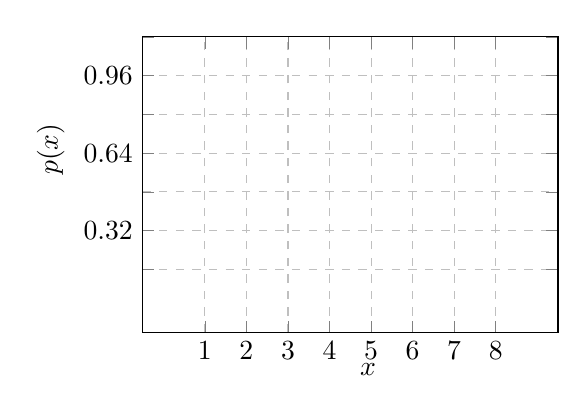
\begin{tikzpicture}[scale=1]
\begin{axis}[
x label style={anchor=west},
xlabel={$x$},
xticklabel style={anchor=north},
y label style={anchor=south west},
ylabel={$p(x)$},
xtick       = {1,2,3,4,5,6,7,8},
xticklabels = {$1$,$2$,$3$,$4$,$5$,$6$,$7$,$8$},
ytick       = {.16,.32,.48,.64,.80,.96,1.12},
yticklabels = { , $0.32$,  ,$0.64$, ,$0.96$, },
samples     = 320,
domain      = -1:9.5,
restrict y to domain=-3.5:2.5,
xmin = -0.5, xmax = 9.5,
ymin = -0.1, ymax = 1.12,
height=2.1in, width=2.7in,
grid=both, grid style=dashed
]
%  \addplot[ name path=f, domain=-.5:2,  blue, ultra thick, <-, ] {0  };
%    \addplot[ name path=f, domain=8:9.5,  blue, ultra thick, ->, ] {1  };
%  \addplot[ name path=f, domain=2:6,  blue, ultra thick, -, ] {.02*x^2-0.08  };
%    \addplot[ name path=f, domain=6:8,  blue, ultra thick, -, ] {-.03*x^2+0.6*x-1.88  };
%    \draw[red,fill=red] (6,0.64) circle (2.pt);
\end{axis}
\end{tikzpicture}
}{
\,
}

\item[(b)] What is the probability that the catch of the day is between 5 and 7 tons?


\vfill
\end{enumerate}



\end{document}

